%-------------------------------------------------------------------------
\section{Comparison and Analysis}
\label{sec:analysis}

This section synthesizes the empirical trends observed in Section~\ref{sec:experiments} and
provides a comparative interpretation of how different positional encoding mechanisms behave under
resolution extrapolation. We focus on four recurring themes: (i) the distinct extrapolation
profiles visible in classification, (ii) the structural difference between additive bias methods
and rotation-based methods, (iii) the contrasting behavior of inference-time frequency scaling
strategies, and (iv) the transfer of these trends to dense prediction tasks.

\subsection{Classification Extrapolation Trends}

The classification results reveal three qualitatively distinct operating regimes as the input
resolution moves away from the training point. In the sub-training regime ($96$--$160$ px), all
methods experience some degradation due to reduced spatial detail, although the extent varies
substantially. In the near-training regime ($224$--$384$ px), several methods improve beyond their
training-resolution accuracy, indicating that higher-resolution inputs can provide genuinely useful
additional spatial information when the positional encoding remains well behaved. In the
far-extrapolation regime ($448$--$1024$ px), the choice of positional encoding becomes the dominant
factor, and the performance gap between methods widens sharply.

\paragraph{Interpolation Regime Anomaly.}
Figure~\ref{fig:interpolation_regime} reveals a surprising finding in the interpolation regime:
ALiBi ViT \emph{collapses} to $1.88\%$ Top-1 accuracy at $96$ px---just $2.6\%$ of its training-resolution
performance---while all other methods retain $36$--$45\%$ accuracy. This asymmetric failure is unique
to ALiBi. We hypothesize that at very low token counts ($6 \times 6 = 36$ patches at $96$ px), ALiBi's
distance-based attention bias becomes \emph{too strong relative to content-based similarity},
effectively overwhelming the learned representations. The bias magnitude scales with distance but
the total spatial extent shrinks, causing disproportionate penalties. At $160$ px ($10 \times 10 = 100$ patches),
ALiBi recovers to $62.2\%$, indicating that the failure mode is specific to very small spatial grids.
This finding has practical implications: ALiBi may require recalibration of slope parameters when deployed at resolutions significantly below the training resolution.

\begin{figure}[t]
    \centering
    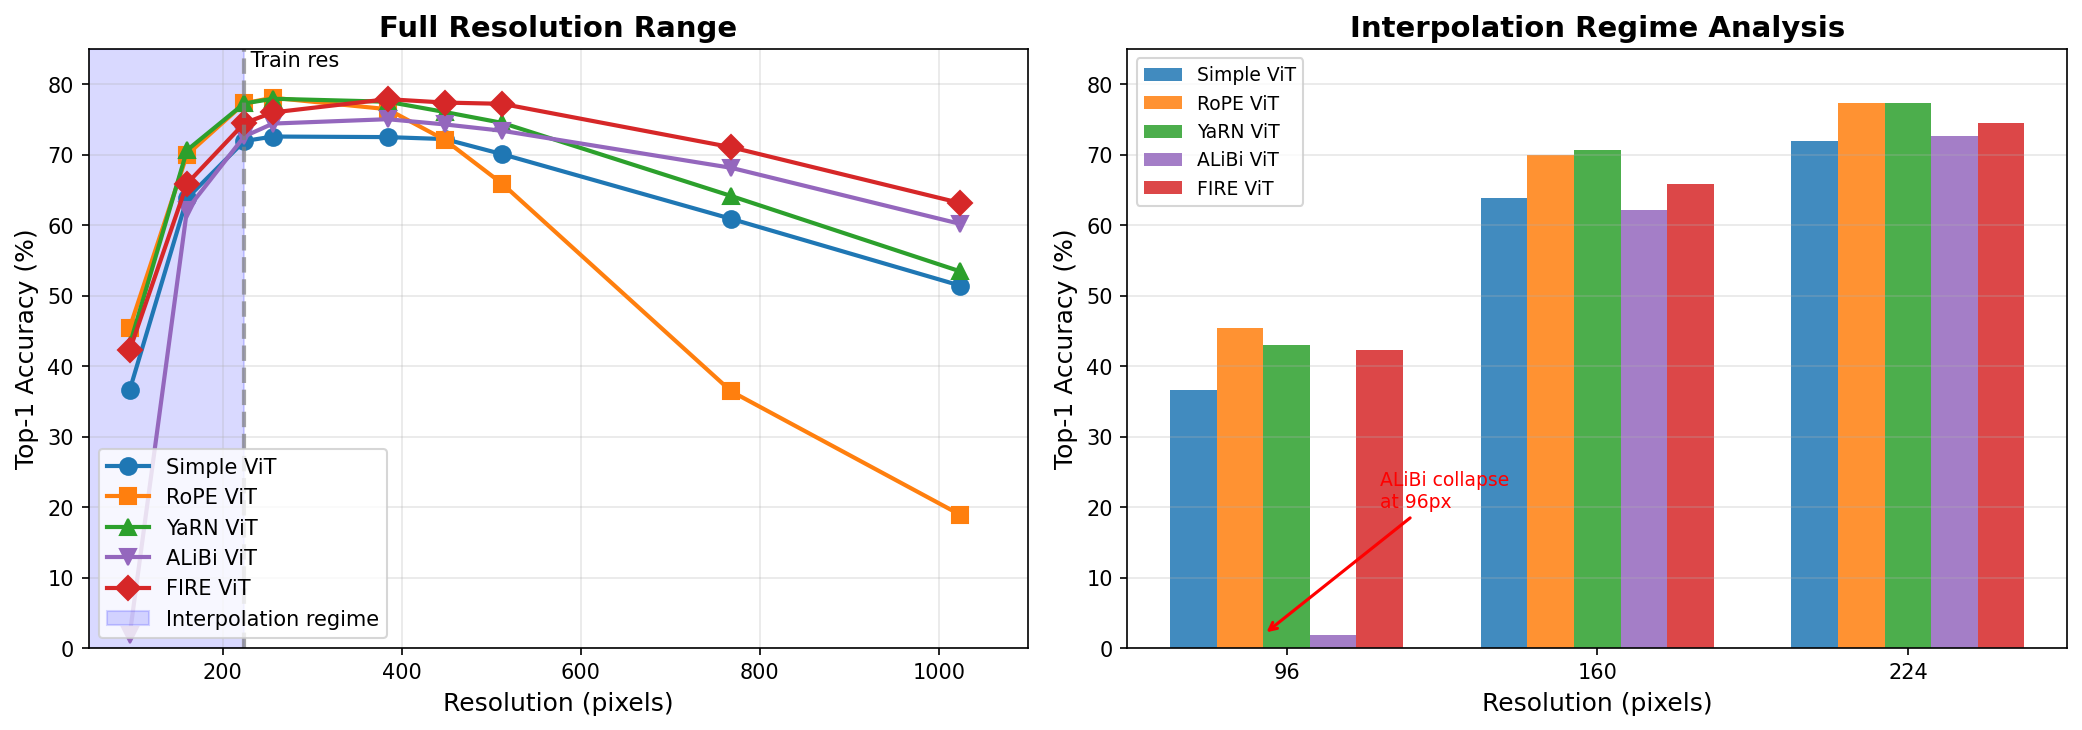
\includegraphics[width=\columnwidth]{figures/interpolation_regime_analysis.png}
    \caption{Interpolation regime analysis. Left: full resolution sweep with interpolation regime highlighted. Right: bar chart of sub-training resolutions showing ALiBi's anomalous collapse at $96$ px ($1.88\%$) while other methods retain $36$--$45\%$ accuracy.}
    \label{fig:interpolation_regime}
\end{figure}

At the largest evaluated scale ($1024$ px, corresponding to $4.57\times$ the training grid), the
Top-1 ranking is: FIRE ($63.14\%$) $>$ ALiBi ($60.18\%$) $>$ YaRN ($53.44\%$) $>$ Simple ViT
($51.42\%$) $>$ RoPE ($18.90\%$). The gap between the
best and worst methods at this scale is $44.24$ percentage points, which is substantially larger
than the $5.36$-point spread at the training resolution ($71.94\%$--$77.30\%$). This demonstrates
that extrapolation robustness, rather than in-distribution accuracy alone, is the primary
differentiator among positional encoding strategies in resolution-flexible Vision Transformers.

The Top-5 curves reinforce the same ordering while showing a slightly more compressed spread. At
$1024$ px, FIRE achieves the highest Top-5 accuracy ($86.80\%$), followed by ALiBi
($84.16\%$) and YaRN ($79.12\%$), while vanilla RoPE drops to $42.94\%$. This indicates that
the strongest methods degrade gracefully: even when the top prediction changes, the correct class
often remains within the top few candidates, suggesting that the underlying representation remains
semantically coherent over a broad range of resolutions. Notably, YaRN's NTK-by-parts scaling
substantially improves its Top-5 retention compared to raw RoPE, nearly doubling it at $1024$ px.

\subsection{Bias-Based vs.\ Rotation-Based Methods}

A consistent pattern across the experiments is the stronger extrapolation behavior of additive
bias-based methods (ALiBi and FIRE) compared to rotation-based methods (RoPE and YaRN).
The key architectural distinction is that bias-based methods inject positional information as an
additive term in the attention logits, whereas rotation-based methods modify the query and key
representations themselves before the dot product is computed.

This difference has important consequences under extrapolation. In bias-based methods, positional
information acts as a spatial prior that encourages locality or relative structure, but the
underlying content-based similarity remains intact. As the resolution increases, the positional
bias simply extends to larger spatial distances, which generally leads to gradual degradation
rather than abrupt failure. This behavior is clearly visible in both ALiBi and FIRE, which remain
strong even at $1024$ px. FIRE is the most robust overall in classification, dropping only
$11.34$ percentage points from its $224$ px Top-1 accuracy ($74.48\%$) to $1024$ px
($63.14\%$), while ALiBi drops only $12.42$ points over the same range.

In contrast, rotation-based methods encode position directly into the geometry of the query--key
interaction. This yields strong in-distribution performance---RoPE achieves the highest Top-1
accuracy at the training resolution ($77.30\%$) and the peak score at $256$ px ($78.08\%$)---but
becomes increasingly fragile when evaluated outside the training range. As the patch grid grows,
the effective positional phases move beyond the range seen during training, and the resulting
attention patterns become progressively less stable. This is most visible in vanilla RoPE, which
falls from $77.30\%$ at $224$ px to $18.90\%$ at $1024$ px, a $58.40$-point collapse.

A notable secondary result is the strength of the Simple ViT baseline. Despite relying on learned
absolute embeddings with bicubic interpolation, it reaches $51.42\%$ Top-1 at $1024$ px,
remaining competitive with YaRN ($53.44\%$) under extreme extrapolation. This
suggests that smooth interpolation of learned absolute embeddings provides a surprisingly strong
``safety floor'' when more sophisticated relative schemes become unstable outside their training
range. However, YaRN's selective frequency scaling enables it to outperform Simple ViT by
maintaining better local spatial precision while still benefiting from interpolated global structure.

\subsection{Attention Pattern Analysis}

To provide direct visual evidence of extrapolation failure, we examine attention maps from the final
transformer layer across resolutions. Figure~\ref{fig:attention_grid} shows CLS token attention
overlaid on a sample image at $224$, $512$, and $768$ px for each positional encoding method.

\begin{figure}[t]
    \centering
    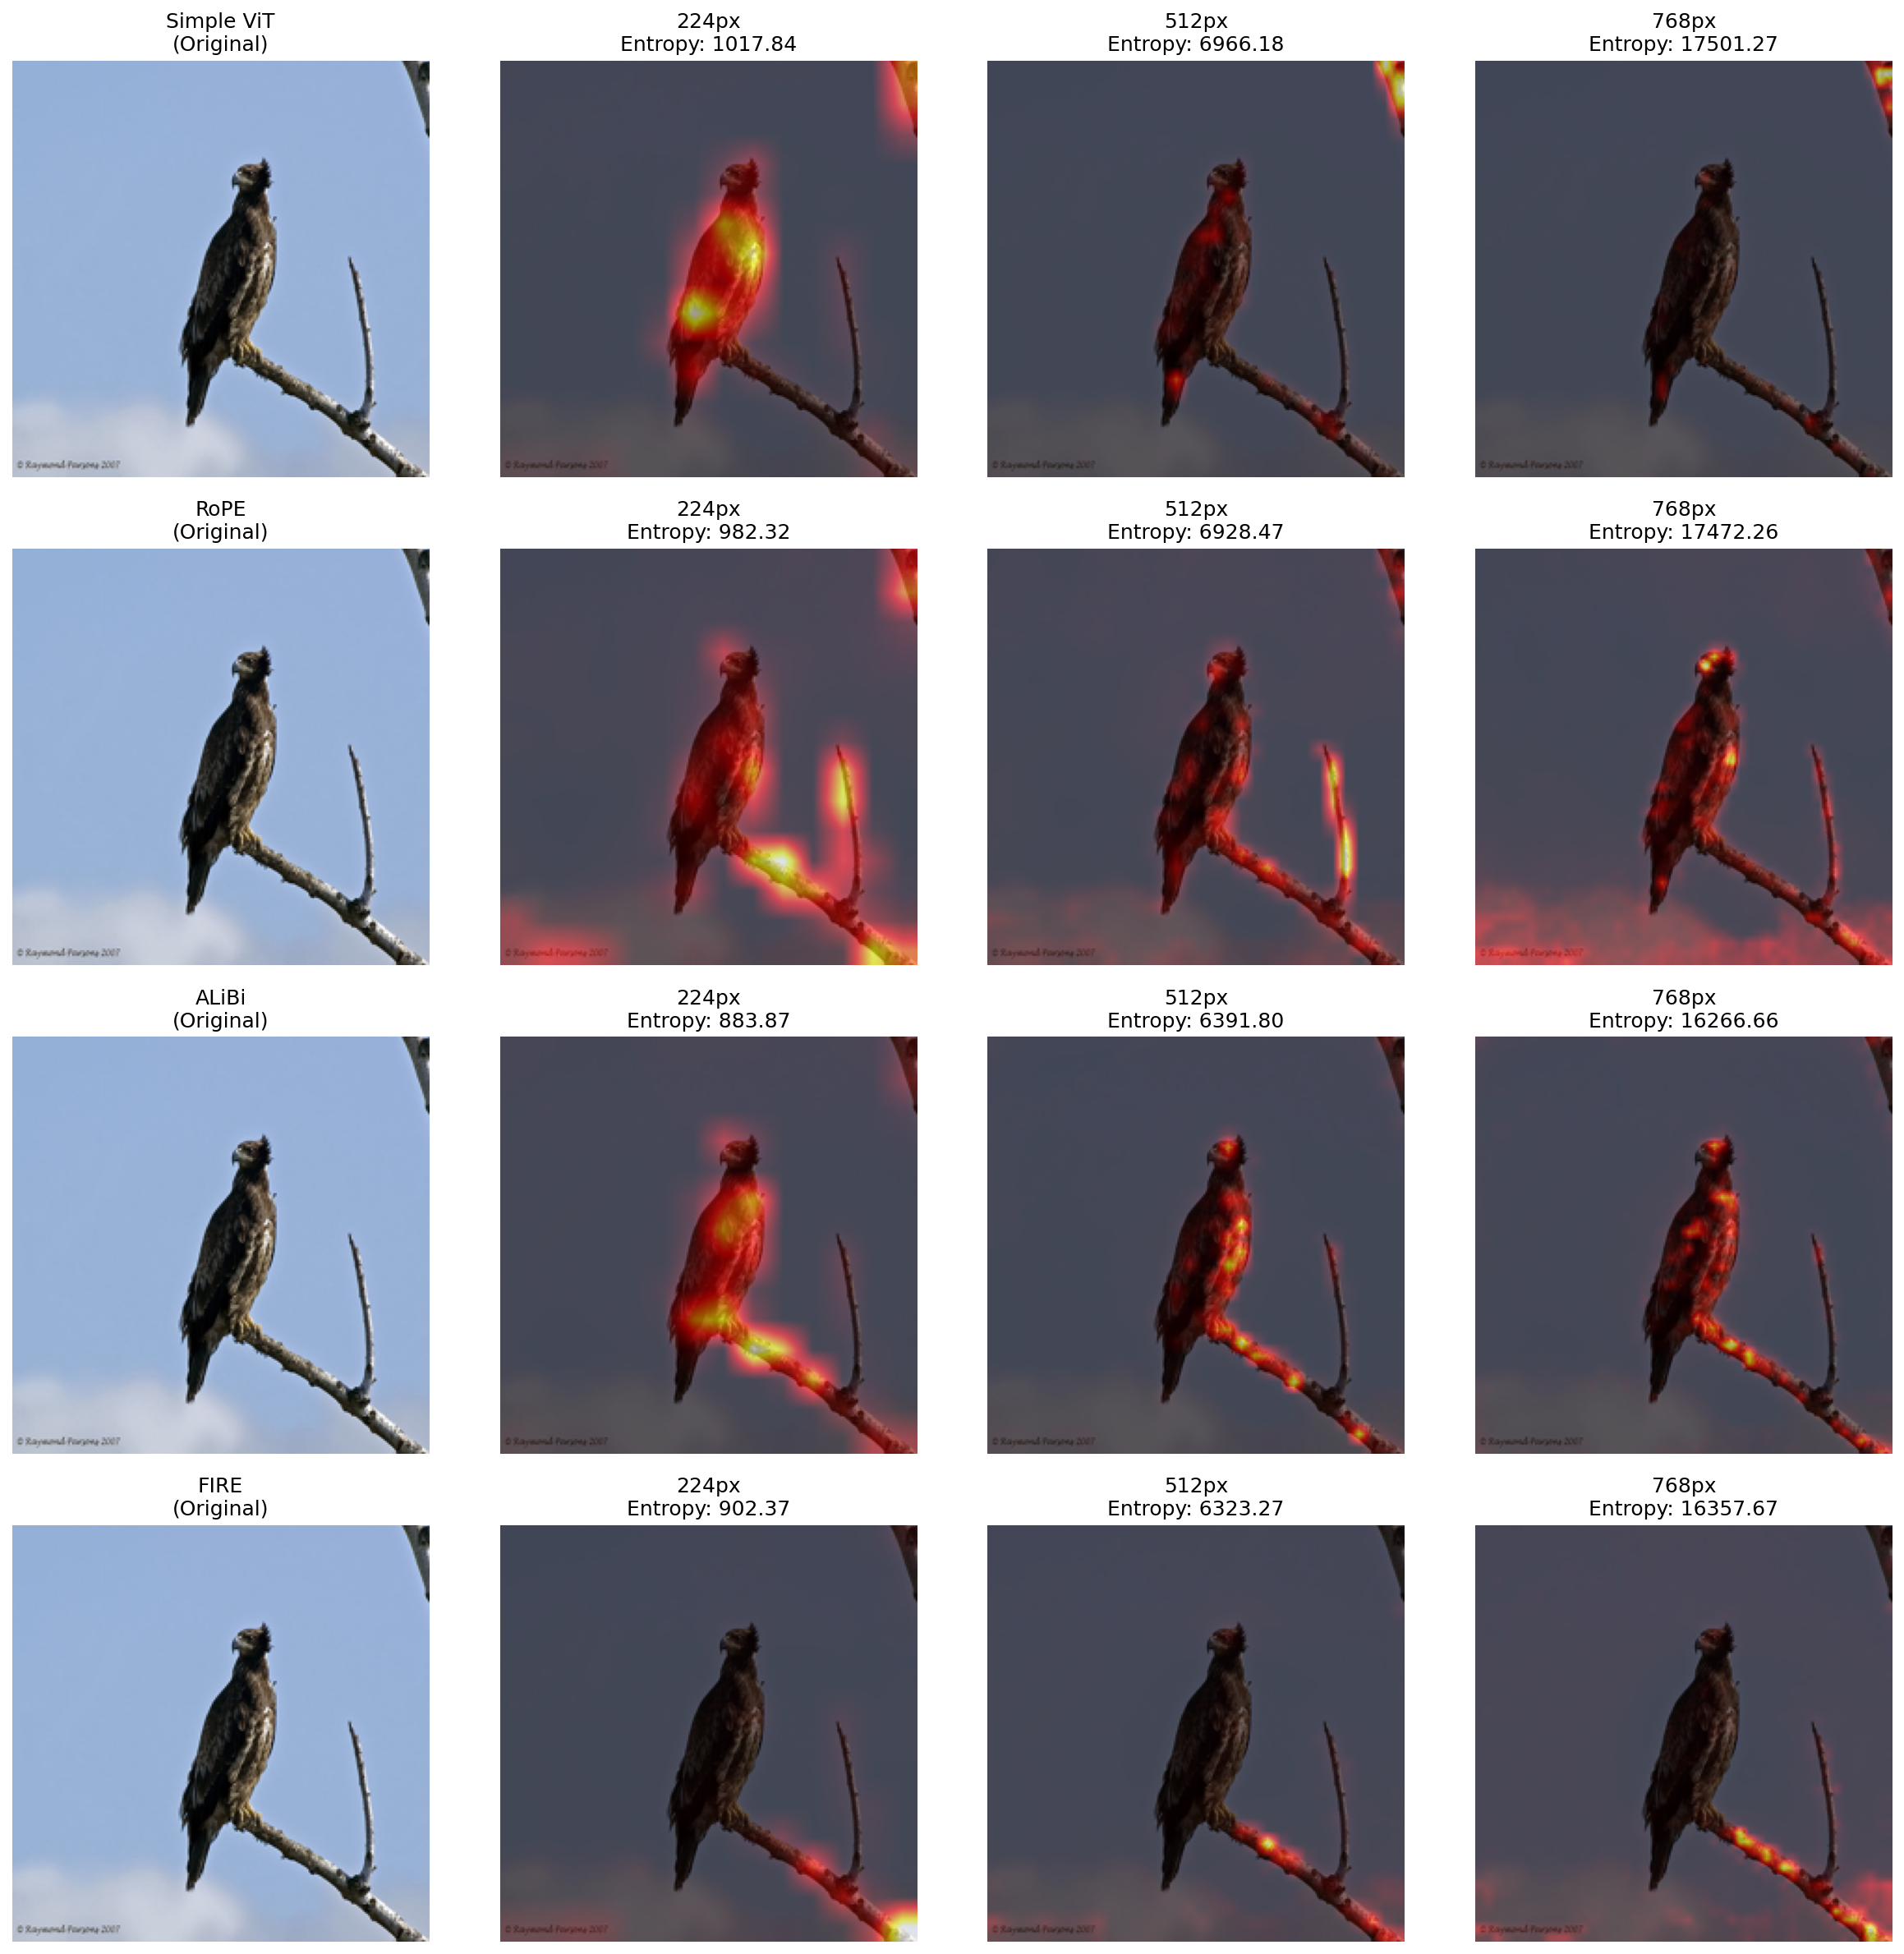
\includegraphics[width=\columnwidth]{figures/attention_visualization_grid.png}
    \caption{Attention visualization across resolutions. Each row shows a different positional
    encoding method; columns show the original image and attention heatmaps at increasing
    resolutions. Attention entropy (summed over all query-key pairs) quantifies attention diffusion.
    ALiBi maintains focused attention at $512$ px (entropy $883.87$) while other methods show
    $6$--$7\times$ entropy increase. By $768$ px, all methods exhibit high entropy, but ALiBi/FIRE
    retain visible concentration on the subject.}
    \label{fig:attention_grid}
\end{figure}

At the training resolution ($224$ px), all methods produce semantically meaningful attention
patterns, focusing on the bird's head and body with entropy values around $900$--$1000$. The
differences become stark at $512$ px: ALiBi's entropy \emph{decreases} to $883.87$, indicating
that its attention becomes \emph{more concentrated} as resolution increases---likely because the
finer spatial granularity allows more precise localization. In contrast, RoPE's entropy jumps
to $6928.47$ ($7\times$ increase), and Simple ViT reaches $6966.18$. Visually, ALiBi's
attention remains tightly focused on the bird, while RoPE and Simple ViT begin attending to
uninformative background regions (sky).

At $768$ px, all methods show elevated entropy ($16000$--$17500$), reflecting the fundamental
challenge of extrapolating to $3.4\times$ the training grid size. However, qualitative differences
persist: ALiBi ($16266.66$) and FIRE ($16357.67$) still exhibit visible concentration on the
subject, whereas RoPE ($17472.26$) and Simple ViT ($17501.27$) produce nearly uniform attention
distributions. This explains why bias-based methods retain reasonable classification accuracy
at extreme scales---even when attention spreads, it maintains \emph{relative} focus on semantically
relevant regions, whereas rotation-based methods lose this spatial coherence entirely.

These attention patterns directly explain the accuracy trends observed in Section~\ref{sec:experiments}:
the graceful degradation of ALiBi and FIRE corresponds to gradually diffusing but still
object-centered attention, while RoPE's sharp accuracy collapse corresponds to attention that
becomes spatially incoherent, effectively treating all image regions as equally relevant.

\subsection{Dense Prediction and Practical Implications}

The dense prediction experiments broadly support the trends observed in classification, but they
also reveal an important nuance: the absolute ranking is not identical across all tasks,
particularly in detection. In object detection, RoPE achieves the highest mAP near the training
regime, reaching $6.8\%$ at $512$ px and remaining strong at $640$ px ($6.0\%$), but it also
exhibits the steepest degradation, falling to $1.5\%$ at $1024$ px. YaRN, applying the same
checkpoint with NTK-by-parts scaling, matches RoPE at $512$ px ($6.8\%$) but degrades more
gracefully to $2.7\%$ at $1024$ px---nearly double RoPE's retained performance. By contrast, ALiBi shows the
most stable detection profile, decreasing only from $3.4\%$ at $512$ px to $2.7\%$ at $1024$ px.
FIRE remains competitive and relatively stable, dropping from $3.4\%$ to $2.3\%$, but under the
current ViT-Tiny setting it does not surpass RoPE in peak detection mAP.

In semantic segmentation, the extrapolation pattern aligns more closely with the classification
results. RoPE achieves the highest score at the training resolution ($25.0\%$ mIoU at $512$ px),
but degrades sharply to $9.2\%$ at $1024$ px. YaRN significantly mitigates this degradation,
retaining $15.4\%$ mIoU at $1024$ px compared to RoPE's $9.2\%$---a $6.2$ pp improvement
from the same checkpoint. By contrast, ALiBi retains $20.5\%$ at $1024$ px,
and FIRE retains $19.8\%$, indicating substantially stronger spatial robustness at large
resolutions. FIRE also exhibits the strongest peak among the stable methods, reaching
$24.4\%$ at $512$ px and remaining above $24\%$ at $640$ px, while ALiBi maintains a flatter and
more consistent curve across the full resolution sweep. YaRN occupies a middle ground,
preserving more spatial coherence than raw RoPE while falling short of the bias-based methods.

These results suggest that positional encoding failures are amplified in dense prediction, where
the model must maintain spatially coherent attention patterns across many local regions rather than
produce a single global classification decision. Classification can partially average out local
errors through the final global representation, whereas detection and segmentation depend more
directly on stable token-to-token spatial relationships. From a deployment perspective, this makes
bias-based methods particularly attractive for multi-scale vision systems: they may sacrifice some
peak in-distribution accuracy, but they provide significantly more reliable behavior when the input
resolution shifts at test time.

Overall, our findings support a clear practical recommendation. If the target application requires
robustness across varying or unseen resolutions, additive bias-based positional encodings---especially
FIRE and ALiBi---offer the strongest trade-off between accuracy and stability. If maximizing
in-distribution accuracy is the primary objective and the evaluation resolution closely matches the
training setup, RoPE remains highly competitive, but its extrapolation fragility should be
carefully considered. YaRN provides a practical middle ground: by selectively rescaling RoPE
frequencies at inference time without retraining, it substantially improves extrapolation
robustness over raw RoPE while retaining much of RoPE's in-distribution strength.

\subsection{Computational Cost}

Table~\ref{tab:compute} reports peak GPU memory and inference throughput across resolutions. All methods have similar parameter counts ($\sim$5.5M), but differ substantially in memory and compute overhead. Bias-based methods (ALiBi, FIRE) require storing the full $N \times N$ attention bias matrix, leading to higher memory at large resolutions---FIRE uses $6.8$ GB at $1024$ px versus $2.8$ GB for Simple ViT. YaRN shows anomalously low memory due to implementation differences in frequency caching. Throughput follows inverse trends: Simple ViT achieves $113$ img/s at $224$ px while FIRE drops to $5.8$ img/s at $1024$ px.

These computational trade-offs should inform deployment decisions. While bias-based methods offer superior extrapolation, their $2$--$2.5\times$ memory overhead at high resolutions may be prohibitive in resource-constrained settings. Conversely, if memory is limited but extrapolation robustness is required, YaRN provides a practical compromise with minimal overhead over RoPE.

\begin{table}[t]
\centering
\caption{Computational cost at varying resolutions (batch size 1). Memory in MB; throughput in images/second. Bold indicates best (lowest memory / highest throughput); underline indicates second best.}
\label{tab:compute}
\small
\begin{tabular}{ll|ccccc}
\toprule
\textbf{Model} & \textbf{Metric} & \textbf{224} & \textbf{384} & \textbf{512} & \textbf{768} & \textbf{1024} \\
\midrule
\multirow{2}{*}{Simple ViT} & Mem. & \underline{38} & \underline{90} & \underline{207} & \underline{901} & \underline{2755} \\
                            & Thr. & \textbf{113} & \textbf{106} & \textbf{106} & \textbf{46} & \textbf{17} \\
\midrule
\multirow{2}{*}{RoPE ViT}   & Mem. & 40 & 96 & 216 & 921 & 2791 \\
                            & Thr. & 80 & 83 & 80 & \underline{36} & \underline{13} \\
\midrule
\multirow{2}{*}{YaRN ViT}   & Mem. & \textbf{35} & \textbf{48} & \textbf{73} & \textbf{195} & \textbf{491} \\
                            & Thr. & 75 & 64 & 67 & 33 & \underline{13} \\
\midrule
\multirow{2}{*}{ALiBi ViT}  & Mem. & 44 & 141 & 362 & 1690 & 5249 \\
                            & Thr. & 99 & 101 & \underline{94} & 28 & 10 \\
\midrule
\multirow{2}{*}{FIRE ViT}   & Mem. & 45 & 165 & 453 & 2165 & 6765 \\
                            & Thr. & \underline{107} & \underline{105} & 84 & 17 & 6 \\
\bottomrule
\end{tabular}
\end{table}